\subsection{Setup}

\noindent We set up the second part of the experiment by loading up the \texttt{w} object into the ROOT session at the beginning, running the following 2 lines of code: \texttt{.L Wenu.C+ \textbackslash \textbackslash\, Wenu w}.\\

\subsection{Verification of electron calibration}

\noindent Next, to verify that the electron calibration from the previous part was applied correctly, we ran the \texttt{FitZee()} command (working similar to the fit function of the previous part) to measure the $Z^0 \rightarrow ee$ mass. Fitting the whole dataset using the \texttt{w.FitZee("")} gave us the plot in Figure \ref{fig:zeeCalib}. This fit gave a weight of the Z-boson as $91.16 \pm 0.01 \,\text{GeV}$. This is close to the true value of $91.1876 \pm 0.0021 \,\text{GeV}$, however the uncertainty in our plot is an order of magnitude larger.\\

\begin{figure}[H]
    \centering
    
\includegraphics[width=\linewidth]{Images/WMASS-Electron_Calibration_1.png}
    \caption{Fit of the $Z^0$ peak of ATLAS data using the electron calibration from the previous part; the mass is determined to be $91.16 \pm 0.01 \,\text{GeV}$}
    \label{fig:zeeCalib}
\end{figure}

\subsection{Inspection of Kinematic Variables}

\noindent With the electron calibration checked, we began plotting the various observables of the `W to e nu' dataset. Using the command (with general syntax)\\

\texttt{w.PlotW("variable", bin-number, lower boundary, upper boundary, "cut selection");}\\

\noindent we obtained a stack plot of the ATLAS data alongside a simulated result. We observed in these plots a mismatch between the simulated and the actual data, as can be seen in Fig. \ref{fig:etmisUnCal} for example, caused due to the QCD background not having been properly normalized yet. To correct for this, we attempted by eye to match the simulated data curve with the curve from the actual `W to e nu' data. This correction was implemented by the command\\

\texttt{w.SetQCDScaleFactor(VALUE));}\\

\noindent where \texttt{VALUE} was determined by us to be the factor $1.85/3.2 \,\times\, 192/225 \approx 0.493$. The corrected graph can be seen in Fig. \ref{fig:etmisCal}.

\begin{multicols}{2}
\begin{figure}[H]
    \centering
    
\includegraphics[width=\linewidth]{Images/WMASS-Background_etmis_uncalibrated.png}
    \caption{\texttt{etmis} (Missing Transverse Energy) data from ATLAS stack plot along with blue dotted curve showing simulated data; the QCD background has not been normalized (i.e. set to a preliminary normalization factor of 1).}
    \label{fig:etmisUnCal}
\end{figure}
\begin{figure}[H]
    \centering
    
\includegraphics[width=\linewidth]{Images/WMASS-Background_etmis_calibrated.png}
    \caption{\texttt{etmis} (Missing Transverse Energy) data from ATLAS stack plot along with blue dotted curve showing simulated data; the QCD background has been normalized.}
    \label{fig:etmisCal}
\end{figure}
\end{multicols}

\noindent With the QCD normalization accounted for, we began looking at the plots of the different variables to identify those sections of it with a low QCD background that we could use for out cut selections later in the experiment. For example, plotting the number of jets (using the property \texttt{njets}), showed us the plot in Fig. \ref{fig:njet}, where the high amounts of QCD background when looking at any number of jets greater than zero informed us that \texttt{njets == 0} was a useful cut we could make. This could be further verified by looking at the plots of other variables when this cut was applied, and noting the high or low amounts of QCD background depending on the cut chosen (see Fig. \ref{fig:jet0} and Fig. \ref{fig:jet4}).

\begin{figure}[H]
    \centering
    
\includegraphics[width=\linewidth]{Images/WMASS-Background_nJet.png}
    \caption{\texttt{njet} (Number of Jets) data from ATLAS stack plot along with blue dotted curve showing simulated data (after QCD normalization); the data for more than 0 jets shows a significant QCD background-to-signal ratio}
    \label{fig:njet}
\end{figure}

% \newpage

\begin{multicols}{2}
\begin{figure}[H]
    \centering
    
\includegraphics[width=\linewidth]{Images/WMASS-Background_Jet0.png}
    \caption{\texttt{el\_pt} (Transverse Momentum of Electron) data from ATLAS stack plot along with blue dotted curve showing simulated data (after QCD normalization); a cut to only show that data where \texttt{njet==0} has been applied}
    \label{fig:jet0}
\end{figure}
\begin{figure}[H]
    \centering
    
\includegraphics[width=\linewidth]{Images/WMASS-Background_Jet4.png}
    \caption{\texttt{el\_pt} (Transverse Momentum of Electron) data from ATLAS stack plot along with blue dotted curve showing simulated data (after QCD normalization); a cut to only show that data where \texttt{njet==4} has been applied, note the greater presence of QCD background}
    \label{fig:jet4}
\end{figure}
\end{multicols}

\noindent Similarly, we attempted to find similar regions in the plots of the other variables which showed a low QCD background which we could use for our cuts, and which showed a prominent Jacobi peak in the \texttt{el\_pt} plot. We finally settled on the following list of cuts: \texttt{njet==0, etmis>35, el\_etiso>1, el\_energy>40}. To apply this on all future fittings of the data, we ran the command\\

\texttt{w.SetCutSelection("cut selection");}\\

\noindent with \texttt{"cut selection"} replaced by the cut parameters we had chosen.\\

\subsection{Gauge curve W-boson mass versus half-maximum point}

\noindent Finally, we applied these cuts on to the different `W to e nu' simulated data sets using the following set of commands (run as a ROOT macro):\\

\noindent \texttt{TCanvas* c1 = new TCanvas("c1");\\
c1->Clear();\\
c1->Divide(4,2);\\
w.SetQCDScaleFactor($1.85/3.2 \,\times\, 192/225$));\\
w.SetCutSelection("njet==0, etmis>35, el\_etiso>1, el\_energy>40");\\
c1->cd(1);w.GetHalfMaximum("MCW75",xmin,xmax);\\
c1->cd(2);w.GetHalfMaximum("MCW78",xmin,xmax);\\
c1->cd(3);w.GetHalfMaximum("MCW79",xmin,xmax);\\
c1->cd(4);w.GetHalfMaximum("MCW80",xmin,xmax);\\
c1->cd(5);w.GetHalfMaximum("MCW81",xmin,xmax);\\
c1->cd(6);w.GetHalfMaximum("MCW82",xmin,xmax);\\
c1->cd(7);w.GetHalfMaximum("MCW85",xmin,xmax);}\\

\noindent These commands create a 4-by-2 subplot of images which are subsequently filled in by the 7 different plots from the 7 different simulated datasets (i.e. the first subplot is of the fit applied to the simulated data with mW = 75$\,$GeV, the second subplot is of the fit applied to the data with mW = 78$\,$GeV, and so on). The QCD Scale Factor setting and cut selections are applied directly in the macro to ensure that any fitting that happens has those set to the values and factors we had previously decided, instead of being affected by any change that may have occurred in the outside ROOT environment.\\

\noindent In each simulated \texttt{el\_pt} plot, a half maximum fit was applied on the data with x-coordinates between \texttt{xmin} and \texttt{xmax}, which we determined by eye to be 30 and 55 respectively for most appropriate fittings, for all the datasets. (The plots are shown in Fig. \ref{fig:allplots} as the first seven subplots. The last two subplots are those of the fits done on the actual `Wenu' and `Zee' datasets, explained ahead. These plots were generated by slightly modifying the above macro to be a 3-by-3 plot instead of a 4-by-2 one.) We thus obtained the value of the half-maximum point for each value of mW given in the datasets. This let us construct a gauge curve relating the two (Fig. \ref{fig:gaugecurve}).

\begin{table}[H]
    \centering
    \begin{tabular}{cc}
        \hline
        mW / GeV&  Half-maximum / GeV\\
        \hline
        75 & 40.97\\
        78 & 42.55\\
        79 & 43.01\\
        80 & 43.51\\
        81 & 44.09\\
        82 & 44.43\\
        85 & 45.90\\
        \hline
    \end{tabular}
    \caption{W-boson masses from the different data sets, and the corresponding half-maxima}
    \label{tab:wgauge}
\end{table}

\begin{figure}[H]
    \centering
    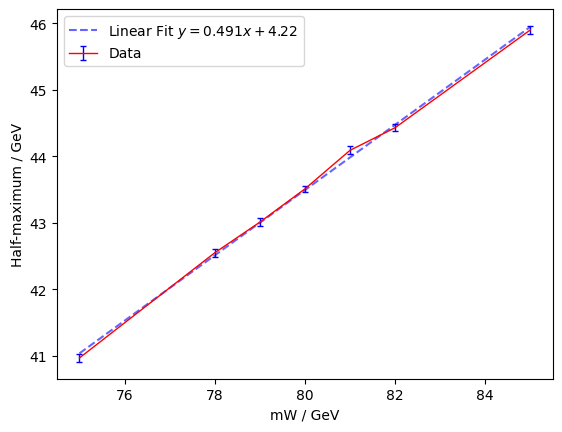
\includegraphics[width=0.7\linewidth]{Images/gaugecurve.png}
    \caption{Above tabular data plotted with error bars, along with a best fit line obtained from \texttt{scipy.curvefit()}}
    \label{fig:gaugecurve}
\end{figure}

\noindent We now applied the fit onto the true dataset \texttt{Wenu}, using the same fit, QCD, and cut parameters, and obtained a half-maximum here of 44.23$\,$GeV (seen as the eighth subplot in Fig. \ref{fig:allplots}). Plugging this into the expression for the gauge curve we fit above gave us a base value for the mass of the W-boson of \textbf{81.50$\,$GeV}.

\noindent Before looking closer at this obtained value to determine the uncertainty in it, we also did a quick check by plotting the fit with the parameters used so far on the `Z to ee' plot, to observe if we obtain the expected Z-boson mass here (the plot can be seen as the ninth subplot in Fig. \ref{fig:allplots}). We got here a half-maximum of 49.74$\,$GeV, which corresponds via the gauge curve to a Z-boson mass of 92.73$\,$GeV, which is close enough to the true mass to show that the parameters we had chosen were quite good.\\

\begin{figure}[H]
    \centering
    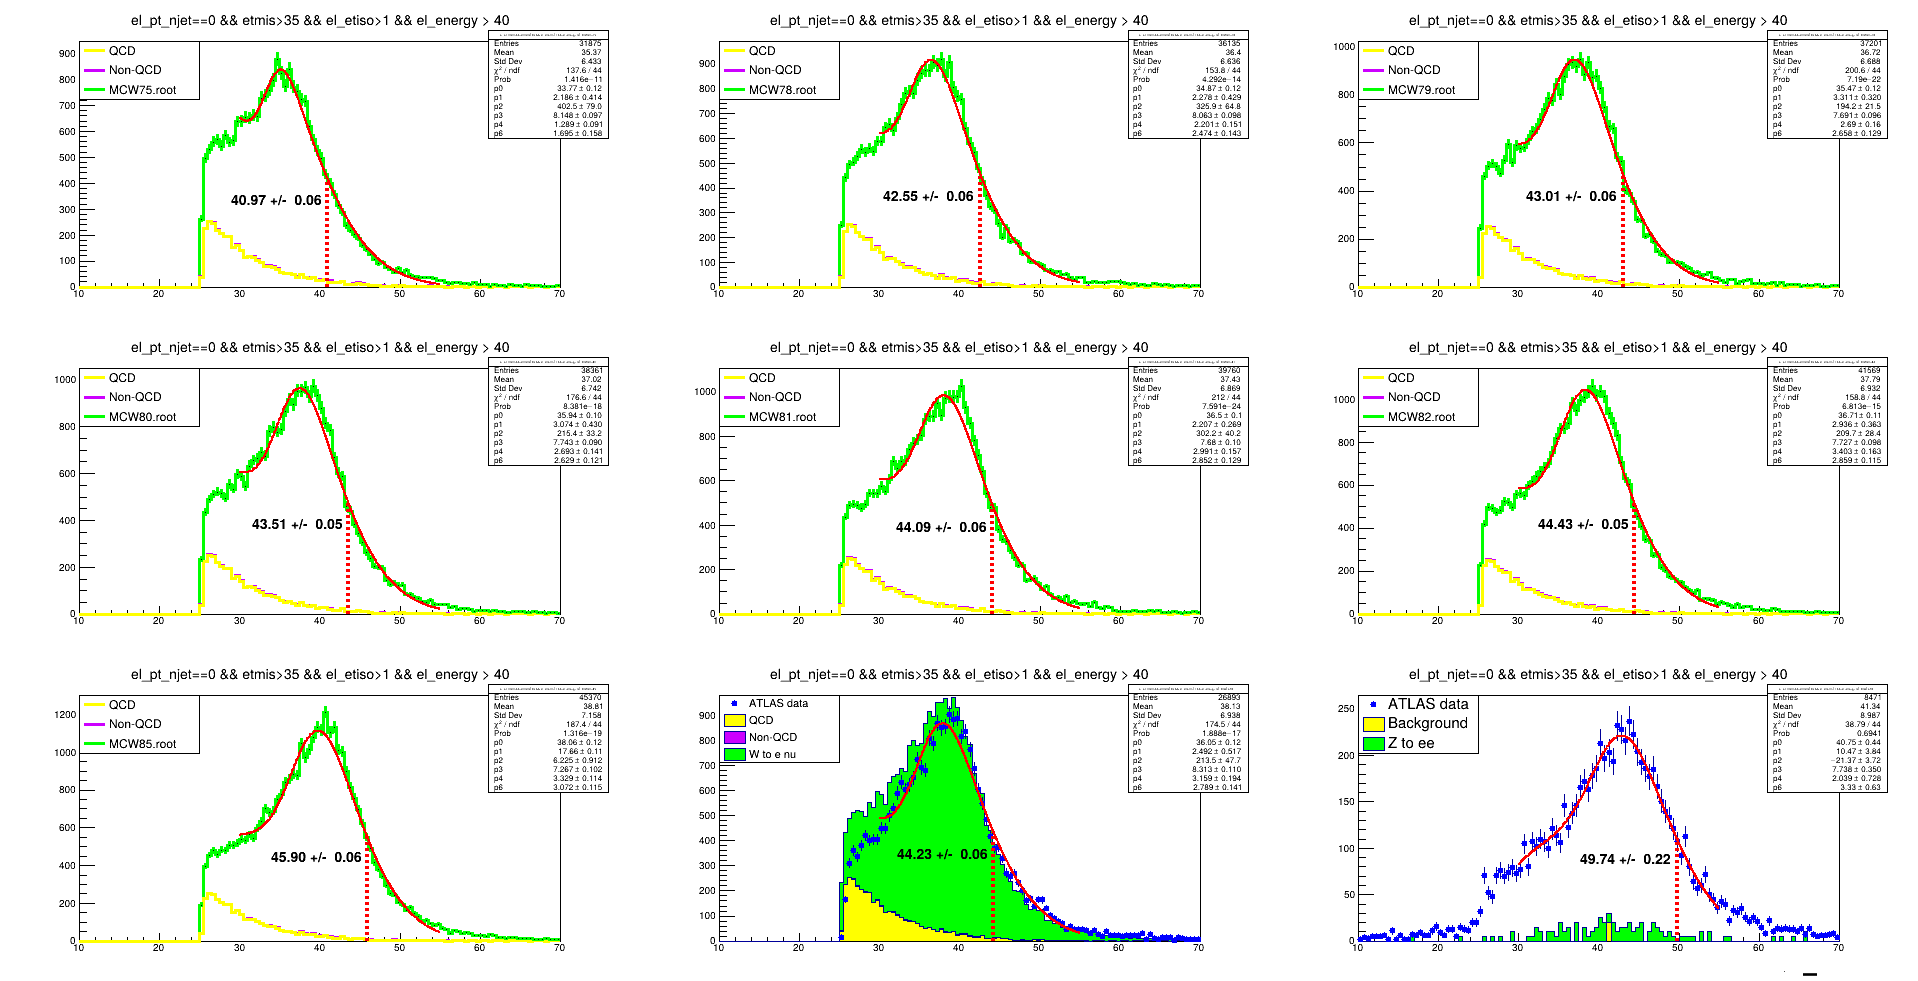
\includegraphics[width=\linewidth]{Images/Wmasses_Wemu_Zee.png}
    \caption{Plots showing the different datasets with the half-maximum fit, each showing the corresponding value. The first seven subplots are for the simulated datasets where the W-boson had a range of masses (listed in the legend of each subplot). The eight subplot is for the actual dataset where the W-boson had its true mass. The ninth subplot is for the Z-boson dataset.}
    \label{fig:allplots}
\end{figure}

\subsection{Other systematic effects and error sources}

\noindent To find the statistical uncertainty in our value of the mass of the W-boson, we used the fit formula obtained above ($\text{half-max} = 0.491 m_W + 4.22$ or rather, this equation flipped to have $m_W$ on one side) and the simple form of Gauss's error propagation law Eq. \ref{gausserr} (i.e. assuming no correlation). This gives us a statistical uncertainty of $1.78\,\text{GeV}$.\\

\noindent For the systematic uncertainty, we approached this by varying the various parameters we had set, first setting them to those values that most loosely fit the data while still being reasonable, then setting them to those values that most tightly fit the data. We changed the cuts we had made, the value of the QCD normalization, and the range of x-coordinates on which the fit was applied. Each set of parameters was changed keeping the other two sets constant. (For the QCD systematic error, when calculating the scale factor by eye originally, we attempted to match the blue dotted curve with the green stack plot as best as we could with reference to the ticks along the Y-axis (see Fig. \ref{fig:etmisUnCal}). When we had settled on a scale factor, we set the least count of the Y-axis at that point as the error, which meant our estimate could've been about $4\%$ greater or less, which is now reflected in this multiplication by 24 (or 26)/25.) The values of $m_W$ that resulted from this are detailed below in Table \ref{systerr}:

\begin{table}[H]
    \centering
    \begin{tabular}{ccc}
        Parameters changed & Change made & $m\_W$ / GeV \\
        
        \hline
        \multirow{2}{*}{Cuts} & \texttt{etmis\textgreater{}25, el\_etiso\textgreater{}0.4, el\_energy\textgreater{}20} (Loose) & $80.89 \pm 1.56$ \\
        & \texttt{etmis\textgreater{}50, el\_etiso\textgreater{}1.4, el\_energy\textgreater{}60} (Tight) & $82.93 \pm 4.46$ \\
        
        \hline
        \multirow{2}{*}{QCD Scale Factor} & $(1.85/3.2 \times 192/225) \times 24/25$ (Loose) & $81.49 \pm 1.78$ \\
        & $(1.85/3.2 \times 192/225) \times 26/25$ (Tight) & $81.52 \pm 1.78$ \\
        
        \hline
        \multirow{2}{*}{Range of x-coordinates} & 25 to 70 (Loose) & $83.29 \pm 2.05$ \\
        & 33 to 50 (Tight) & $81.10 \pm 2.95$ \\
        \hline
    \end{tabular}
    \caption{The variation of the various parameters to a loose and tight extent, along with the corresponding resulting calculations for the mass of the W-boson.}
    \label{systerr}
\end{table}

\noindent As can be seen, the variation in the QCD scale factor changes the measured W-boson mass very little, with both these values and our original value lying comfortably within their uncertainties. Changing the cuts and the range of x-coordinates changes the values of $m_W$ a little more, but again, they are close enough to our original value to not fall outside the uncertainties.\\

\noindent Finally, comparing the value we obtained to the expected value of $80.403\pm0.029\,\text{GeV}$, we see that this value lies within the statistical uncertainties we calculated. So, our measured value of $m_W = 81.50\pm1.78\,\text{GeV}$ is good reproduction of the true, expected value.\\